\documentclass[11pt]{article}
\usepackage[margin=1in]{geometry}
\usepackage[T1]{fontenc}
\usepackage[utf8]{inputenc}
\usepackage{lmodern}
\usepackage{amsmath,amssymb,amsthm}
\usepackage{booktabs,array,longtable}
\usepackage{graphicx}
\usepackage{enumitem}
\usepackage{xcolor}
\usepackage{hyperref}
\hypersetup{colorlinks=true,linkcolor=blue,urlcolor=blue,citecolor=blue}
\def\UrlBreaks{\do\/\do\_\do\-\do\.}
\setlength{\emergencystretch}{2em}
\newcommand{\artifact}[1]{{\small\path{#1}}}
% Include this file once, then call the two macros where desired.
% Requires amsmath and amssymb. Uses only standard \cite commands.
\newcommand{\DecisionLeverageTheory}{%
\section{A finite-support decision audit}
\label{sec:decision-audit}

\paragraph{The object being audited.}
An audit context $x$ fixes a physical root state, task goal, executable
candidate bank $\mathcal A_x=\{a_1,\ldots,a_K\}$, horizon, continuation
policy, observation encoding, and utility definition. A candidate may be
an action chunk; its continuation must be the same under every comparison.
Let $u_k=U(x,a_k)$ be its utility measured by environment execution.
Higher utility is better, so a cost is negated before applying the definitions.
Success, return, terminal reward, and time-to-completion are distinct
utilities and receive separate audits. Initially, $u_k$ denotes a fixed
cached outcome; the extension to expected outcomes is given below.

The model supplies forecasts $\widehat z=(\widehat z_1,\ldots,\widehat z_K)$.
A frozen scoring and selection rule $\sigma$ produces a distribution
$p=\sigma(\widehat z)$ on the bank; deterministic selection is a point mass.
We write $U(p)=\sum_k p_k u_k$. The audited intervention may replace the
forecast supplied to this selector. It must not change the task goal,
candidate actions, root state, scoring parameters, continuation policy,
utility implementation, or the coupling of random streams. A system whose
native policy does not consume forecasts can be studied only through a
separately identified, added planner. Neither kind of audit establishes an
adversarial attack without a specified feasible intervention and observed
utility loss.

\subsection{Leverage and baseline-relative harmful headroom}
Define
\begin{align}
 u_{\max}&=\max_k u_k, &u_{\min}&=\min_k u_k,\nonumber\\
 \mathrm{Lev}(x)&=u_{\max}-u_{\min}, &
 H_b(x)&=U(p_b)-u_{\min},
 \label{eq:leverage}
\end{align}
where $p_b$ is the baseline selector. The first quantity is the width of
the feasible utility interval. The second is the maximum loss relative to
this baseline when unrestricted selection within the recorded bank is
allowed; a constrained intervention can attain less.

\paragraph{Proposition 1 (finite-support bound).}
For any two distributions $p,q$ on the same bank,
\begin{equation}
 |U(p)-U(q)|\leq \mathrm{Lev}(x)\,\mathrm{TV}(p,q)
 \leq\mathrm{Lev}(x),\qquad
 U(p_b)-U(q)\leq H_b(x),
 \label{eq:bound}
\end{equation}
where $\mathrm{TV}(p,q)=\tfrac12\sum_k|p_k-q_k|$.
For a panel with nonnegative weights $w_x$ summing to one, the corresponding
aggregate upper bounds are the weighted sums of these bounds.

\paragraph{Proof.}
Subtract $u_{\min}$ from every utility; the difference of expectations is
unchanged because both distributions sum to one. On coordinates with
$p_k>q_k$, the positive contribution is at most
$(u_{\max}-u_{\min})\sum_{p_k>q_k}(p_k-q_k)$; negative contributions
cannot increase it. This sum is $\mathrm{TV}(p,q)$. Interchanging $p$ and
$q$ gives the absolute bound. Every expectation is at least $u_{\min}$,
which gives the baseline bound. Nonnegative weighted summation preserves
the inequalities. Selecting an extreme-utility candidate attains the
interval endpoints when unrestricted selection is permitted.\hfill$\square$

These inequalities are elementary consequences of finite support, not a
new robustness theorem. Their use is to check whether an interface can
exhibit a practically meaningful effect before spending model calls.
They require real branch outcomes, and are therefore not free to compute
when the cache does not yet exist. A deterministic top-choice flip is
necessary for a utility change on this bank, but a flip between equal-utility
candidates has zero effect. Changes in lower ranking positions are weaker
evidence still. A bound violation calls for checking candidate coverage,
continuations, replay randomness, and utility definitions; it does not
refute the finite-support identity. A small bound on one bank is not a
guarantee about unrecorded actions, later replanning, or other states.

\paragraph{Averaging actions is not randomizing over actions.}
If a planner executes an elite mean $\bar a=\sum_k w_k a_k$, its utility is
$U(x,\bar a)$, not $\sum_k w_k U(x,a_k)$. For example, the constructed
utility $U(a)=a^2$ gives utility one for both recorded actions $-1$ and $1$,
but zero for their mean. Thus their recorded leverage is zero while the
unrecorded mean loses one unit. The actual mean must be replayed and
included in the support; changes in an adaptive CEM search distribution
are also outside a frozen-bank bound unless their outputs are covered.

\subsection{A signed true-future comparison}
Let $z^\star$ be the encoding of the real future for each recorded
candidate, at the same prediction horizon and with identical preprocessing.
Keep the scorer and tie-breaking rule fixed and define
$p^\star=\sigma(z^\star)$. Then
\begin{align}
 \mathrm{Reg}(x)&=u_{\max}-U(p),\nonumber\\
 \mathrm{Mis}(x)&=u_{\max}-U(p^\star),\nonumber\\
 \mathrm{Pred}(x)&=U(p^\star)-U(p),\nonumber\\
 \mathrm{Reg}(x)&=\mathrm{Mis}(x)+\mathrm{Pred}(x).
 \label{eq:decomposition}
\end{align}
The identity follows by adding and subtracting $U(p^\star)$.
$\mathrm{Mis}\geq0$ is the residual regret of the frozen
representation--scorer--selector interface when supplied encoded true
futures. It need not be solely a scorer-weight defect: lossy representations,
horizon mismatch, utility-proxy mismatch, ties, and an approximate selection
rule can all contribute. Encoded true futures do not provide a perfect
physical state representation or the optimal full-horizon planner.

In contrast, $\mathrm{Pred}$ is signed. A negative value means that model
forecasts select a higher-utility candidate than true-future substitution
does. It can reflect compensating errors. The two terms must not be
presented as nonnegative shares of an error budget. The algebra alone also
does not identify causal mediation through a complete native planner:
it is a controlled replacement comparison at a declared frozen interface.
True futures are an offline diagnostic and cannot be used as an available
deployment input or as labels for a test-set-trained defense.

\paragraph{Two constructed examples clarify the claims.}
Take two actions with utilities $(1,0)$ and a selector maximizing $-z_k$.
If the true features are $(0,1)$ but the model predicts $(1,0)$, then
$\mathrm{Mis}=0$ and $\mathrm{Pred}=1$: prediction error causes regret
despite a correctly ordered true-future proxy. Objective mismatch is
therefore not a necessary condition for predictive error to harm decisions.
Conversely, if the true features are $(1,0)$ and the model predicts
$(0,1)$, then $\mathrm{Mis}=1$, $\mathrm{Pred}=-1$, and
$\mathrm{Reg}=0$. Replacing the forecast with the truth reduces its squared
prediction error to zero but decreases utility. These are mathematical
counterexamples, not experimental results from any audited model.

\paragraph{Forecast error is different from goal cost.}
Forecast error compares $\widehat z_k$ with the real consequence
$z_k^\star$ of the \emph{same} action. Distance between an encoded outcome
and a desired goal is a planning cost, even when both quantities are called
visual MSE. A lower goal distance together with lower task return
demonstrates proxy disagreement; it does not establish improved predictive
fidelity. In particular, $\mathrm{Mis}>0$ alone does not prove the hypothesis
that improving forecasts makes decisions worse.

\subsection{Uncertainty and identifiable follow-up tests}
For a stochastic environment, replace $u_k$ by
$\mu_k=\mathbb E[U(x,a_k)]$ to obtain a population statement for the
\emph{fixed} bank and continuation. A single replay only supplies a realized
outcome; its empirical extrema do not bound these expectations. If
simultaneous intervals $[\ell_k,r_k]$ cover all $\mu_k$ with probability
at least $1-\alpha$, then on this event
\begin{equation}
 \mathrm{Lev}_{\mu}\leq\max_k r_k-\min_k\ell_k,
 \qquad
 H_{b,\mu}\leq\sum_k p_{b,k}r_k-\min_k\ell_k.
 \label{eq:uncertain-bound}
\end{equation}
For bounded returns in $[A,B]$ and $n_k$ independent replications per
candidate, one elementary construction uses sample means plus or minus
$(B-A)\sqrt{\log(2K/\alpha)/(2n_k)}$, clipped to $[A,B]$.
This follows from Hoeffding's inequality~\cite{hoeffding1963bounds} and a
union bound. The within-arm
independence assumption is necessary; shared random numbers across arms
do not themselves invalidate the union bound. Reusing one realized future
both as an oracle selector input and its evaluation can yield a clairvoyant
choice; it is not the expected performance of an implementable policy.
Scoring an expected latent is also generally different from averaging
scores of stochastic futures.

A fidelity--utility reversal test must compare two specified forecast
inputs on identical candidates, show an improvement under a preregistered
forecast-error metric, and measure a decrease in independently evaluated
selected-action utility. An offline interpolation toward true futures can
test that interface property, but cannot claim a deployable accuracy
improvement. Establishing positive mean $\mathrm{Mis}$ is a separate test
of residual regret. Establishing that scorer repair outperforms forecast
repair requires a direct, paired comparison of held-out utilities under
both interventions, together with their unmodified controls. The identity
does not predict which feasible repair will win. Calibration roots,
model or metric selection, and final evaluation roots must be separated.
Independent episode or initial-state clusters, rather than candidates or
multiple roots from the same episode, determine the sampling unit. Thirty
roots is a possible design size, not a guarantee of power; uncertainty and
minimum detectable effect depend on variability and the sampling design.
}

\newcommand{\DecisionLeverageRelatedWork}{%
\section{Related work and contribution boundary}
\label{sec:related-work}

\paragraph{Prediction quality and decision quality.}
Lambert et al.~\cite{lambert2020mismatch} identify objective mismatch in
model-based reinforcement learning and empirically show that one-step
prediction likelihood need not track downstream control performance.
Consequently, better prediction together with worse control is not a new
principle or discovery of this study.
Smart Predict-then-Optimize measures errors through the decisions they
induce rather than through a prediction loss alone~\cite{elmachtoub2022spo}.
Value-aware model learning and value equivalence adapt environment models
to their downstream value calculations~\cite{farahmand2017vaml,grimm2020value}.
TEMPO incorporates task-aware sample weighting into model
training~\cite{yuan2023tempo}. These precedents rule out treating the
general distinction between predictive accuracy and control utility as
our novelty. We instead operationalize a finite-support audit for frozen
interfaces and existing branch-replay artifacts, then examine a fixed additive
forecast correction and its horizon-dependent effect in a native CEM query.

\paragraph{Objective proxies.}
Pan et al.~\cite{pan2022misspecification} study cases in which stronger
optimization of a proxy accompanies lower true reward. Our true-future
comparison concerns a frozen planning proxy and a specified candidate
bank, and does not establish deliberate reward hacking. The residual
regret in Eq.~\eqref{eq:decomposition} also includes representation and
selection limitations. Adding and subtracting an oracle-interface utility
is an accounting identity, rather than a new causal identification theorem.

\paragraph{Model exploitation and security claims.}
Bhamidipaty et al.~\cite{bhamidipaty2026exploitable} define model exploitation
through opposite policy orderings under model and environment dynamics
(Section 2.2), and explicitly discuss an optimizer producing such behavior
without an external adversary (Section 1). This is close prior work for
interpreting ordering disagreements. Our goal-feature scorer is not itself
an estimate of task return, so proxy disagreement should not be conflated
with their transition-model definition. Neither an ordering reversal nor
the generic prediction--control mismatch establishes a new security mechanism.
Such a claim would additionally need a specified feasible external intervention
and measured real-utility consequences under that intervention.

\paragraph{Visual world-model planning.}
DINO-WM plans toward goal features using an action-conditioned latent
predictor~\cite{zhou2024dinowm}. Cosmos Policy jointly represents actions,
future observations, and values, and uses their predictions for
planning~\cite{kim2026cosmos}. Their different consumers motivate checking
the actual action-selection interface before interpreting forecast changes.
CF-JEPA separates controllable and uncontrollable latent components,
whereas Dueling World Models centers predictions across actions to expose
an action-dependent channel~\cite{byrd2026cfjepa,li2026dueling}.

The publicly available LENS submission abstract describes a frozen-model
planning metric derived from real/predicted action-response agreement and
prediction accuracy, including a fixed-candidate, fixed-prediction ranking
comparison~\cite{anonymous2026lens}. This directly overlaps the idea of
reweighting latent directions to improve action rankings. We verified its
official abstract and submission metadata, but could not access its full
text; its reported performance is not evidence from our experiments.
Consequently, we make no priority claim for latent reweighting, forecast
versus decision evaluation, or oracle subtraction. The contribution sought
here is a reproducible interface audit with explicit support, replay
provenance, and claim-specific evidence. Its empirical scope is determined
by the audited results, not by the number of model repositories archived.
}

\title{Forecast Accuracy, Decision Leverage, and Objective Mismatch\\
in World-Model Planning}
\author{Research manuscript}
\date{16 October 2026}

\begin{document}
\maketitle
\begin{abstract}
Evaluating a world model by forecast error alone leaves two decision-level
questions unanswered: how much can the evaluated selection interface change
real outcomes, and would its scorer choose well even with actual future
observations? We operationalize these questions with a finite-support utility
audit and an oracle-feature scoring diagnostic. On 30 recorded Cosmos Policy
development roots with two first-action continuations each, any selector over
that fixed support attains between 28 and 30 successes. Relative to the recorded
29-success controller, first-choice-only damage is at most one additional
failure, although completion cost retains more variation. A prospective DINO-WM
reproduction experiment evaluates an added ranker over five frozen development
action sequences on 30 independently reset MetaWorld reach roots. Replacing
predicted features with actual-future encodings lowers mean 30-control terminal
reward from 6.300613 to 4.758220: paired mean change $-1.542393$, with a
95\% bootstrap interval of $[-2.438788,-0.715561]$. Reward decreases at 11
roots, ties at 18, and improves at one. Oracle forecast error is zero by
construction, a manipulation check rather than a deployable forecasting
improvement. Fixed choices of candidate0 and candidate2 achieve higher mean
terminal rewards, 7.306371 and 7.262187, than the original ranker. A separate
development example shows an oracle-feature ordering that no nonnegative,
nonzero reweighting of the scorer's two components repairs. Exploratory reuse
of the 30 roots with a frozen, development-fitted additive bias also lowers
forecast MSE and selected utility. In a separate single-root native CEM query,
the same correction lowers 15-control reward and return, but improves both
over the returned mean's 30-control open-loop continuation. A complete native
replanning episode at that same root raises 99-control return from 747.432862
to 760.171563, failing the preset persistent-loss gate, although first success
is delayed from control 72 to 97. The evidence supports
interface-specific diagnoses of a known prediction--control mismatch, with
explicit baseline-competence and scope limitations; it does not establish
an attack, a validated defense, or cross-task generality.
\end{abstract}

\section{Introduction}
World-model planning inserts a prediction between an action proposal and an
action choice. An evaluation can consequently fail in several distinct ways:
the available actions have nearly identical task outcomes; predicted futures
are inaccurate; the scorer rewards the wrong aspects of even an accurate
future; or a change to the prediction also changes which actions are proposed.
Forecast divergence and action-rank changes do not identify which of these
explanations applies. Actual environment outcomes and an explicit decision
interface are necessary to separate them.

The distinction between prediction accuracy and decision quality is established
in decision-focused learning and model-based reinforcement learning, including
Lambert et al.'s objective-mismatch study~\cite{lambert2020mismatch}. We do
not propose ``better prediction, worse control'' as a new discovery. Our question is operational: what can be
established from the interfaces and real continuation caches of existing
pretrained world-model systems, without retraining a large model or labeling
every changed forecast as a successful attack?

We study two complementary diagnostics. First, a complete finite candidate
continuation table bounds the outcomes reachable by a selector restricted to
that table. The useful quantity for harm is not just the range of outcomes,
but the downside relative to the particular baseline being evaluated. Second,
feeding the measured future representation to the same scorer tests whether
prediction perfection on that bank would remove its regret. This substitution
does not make the representation, objective, or candidate set perfect.

The results are intentionally tied to measured interfaces. The Cosmos audit
contains 60 real continuations at 30 development roots. The prospective DINO
diagnostic evaluates the same five frozen development action sequences at each
of 30 fresh, independently seeded roots, using an added fixed-bank ranker.
Earlier two-mean and five-action development diagnostics retain their exploratory
status and are not pooled with the confirmation panel. A subsequently designed
fixed-bias correction reuses the 30 roots and is therefore exploratory; a
separate single-root native CEM comparison tests its execution-prefix effect
and exposes a reversal under longer open-loop execution. A complete native
episode then reuses that inspected root and finds higher cumulative return
with the correction; it is a further exploratory check, not another independent
root. WorldAgen's corrected short replays are an
interface control because its frozen native policy does not rank world-head
forecasts. Resource availability in additional systems is not empirical
coverage of these tests.

Our contributions are a reproducible finite-cache evaluation procedure, an
explicit account of the assumptions needed to connect it to a planner, and
two measured diagnoses that alter the interpretation of earlier experiments,
including an independent-root confirmation of an offline oracle-substitution
effect within a prespecified fixed bank.
The bounds and regret identity are elementary tools, not claimed new theorems.
The substantive empirical question---how commonly prediction improvements
decrease task utility in independently sampled native planning queries---
remains open: the oracle confirmation does not regenerate native CEM proposals,
the deployable-form correction reuses examined roots, and the native
follow-ups cover only one root, with opposite short-prefix and complete-episode
utility directions and no full-episode forecast-fidelity audit.

\DecisionLeverageRelatedWork

\DecisionLeverageTheory

\section{Evidence, systems, and evaluation protocol}
\label{sec:protocol}
\subsection{Evidence provenance}
This study combines archival reanalysis with a completed prospective experiment.
The Cosmos panel aggregation and development objective-weight audit reuse saved
model outputs and continuations without new inference or environment stepping.
The DINO confirmation panel instead executes 150 candidate continuations at
30 new roots: 4500 candidate controls, 30 forecast unrolls, and 240 encoding
calls. Its recorded CPU invocation takes 897.12 seconds, loads the model once,
and makes no model API calls, network attempts, training updates, or CUDA calls.
The separate expert-goal setups and root warmups add 3000 and 30 explicit
controls; constructor-internal simulation is not instrumented. Subsequent
aggregation uses cached outputs. Four later diagnostics are distinguished
from this confirmation: R003 executes one native CEM query and 165 candidate
prefix controls; R004 phase 1 fits and evaluates a fixed bias entirely from
caches; and R004 phase 2 executes two native CEM queries and 60 replay controls
at a separate root. R004 phase 3 runs complete native episodes at that same
root, with 14 planning queries and 198 policy controls across the two arms.
Its worker completes in 343.45 seconds and records a sampled process peak of
5710 MiB. Each native diagnostic has an expert-goal setup and warmup, with
phase 3 reproducing phase 2's root and Goal exactly. These exploratory
follow-ups are not additional confirmation roots for the original oracle test.
R005 separately crosses saved TD-MPC2 dynamics modules between their native
proposal and evaluation roles, executing four complete 500-control episodes
in 90.68 seconds without training or API calls. This is one reused development
case, not four independent roots or a new attack.
Sources and recomputation entry points appear in Appendix~\ref{sec:artifacts}.
We retain technical failures, stopped gates, and protocol corrections as such,
rather than counting them as failed tasks or silently replacing their results.

Only measurements with an identified root, fixed candidate identity, declared
continuation, and independently measured physical utility can enter a utility
support table. Model values, latent distances, and predicted rewards cannot
serve as the ground truth. A table may be complete for a restricted interface
without being complete for the planner's action space.

\subsection{Cosmos Policy: a fixed first-choice interface}
The audited implementation uses a candidate--future--value path: generate an
action candidate, predict a future conditional on it, and score that future
before selecting a candidate. The development panel contains ten LIBERO-Goal
tasks with three initial states per task. For each root, both saved first
candidates have real continuations. The selected first block contains 16
physical controls; subsequent planning uses the original task Goal and the
recorded native continuation settings. The horizon cap is 300 controls.

We evaluate success and capped completion steps separately. Cost is converted
to utility by sign reversal where needed in the formal definitions. A success
tie does not imply a cost tie. The panel has a deterministic recorded outcome
for each branch; it is not a confidence bound on repeated stochastic rollouts.
Tasks are the natural grouping variable for any exploratory uncertainty
calculation. Thirty roots and sixty branches do not supply sixty independent
replicates.

The Goal-Swap diagnostic changes only the Future branch's text, while the
Policy and Value branches retain the original task. We distinguish a
cache-derived first-choice contrast from a separately executed continuous-Swap
episode. A join that selects an already measured continuation is an offline
evaluation, not a newly executed recovery episode. The local Torch compatibility
adapter also remains part of the evaluated implementation; these measurements
do not establish parity with every upstream numerical backend.
This is a researcher-controlled internal Future-context intervention.
A legal alternative Goal in the same scene does not establish an externally
writable interface, joint training-support membership, or a universal
Goal-invariance obligation for observational predictions.

\subsection{DINO-WM reproduction: fixed action banks}
Our checkpoint and planner come from the JEPA-WMs project's DINO-WM
reproduction~\cite{terver2025drivessuccessphysicalplanning}.
The native planner uses CEM with 300 samples, 15 iterations, 10 elites, six
macro-actions per plan, and five physical controls per macro-action. It
normally executes three macros before replanning. The task Goal is used in
the scoring objective; it is not a separate Goal field in this action-conditioned
predictor. Thus the operation here is not Goal-Swap.

The historical two-action diagnostic fixes the first complete mean returned by each of
two native planning conditions as $a_0$ and $a_1$. These means were selected
post hoc and replayed from the same root for all 30 controls. The first 15
controls match the saved native prefixes. The remaining controls are an
open-loop suffix, not the replanning behavior that the native controller would
have executed. They form a newly evaluated two-action bank, not the native
300-sample population. In particular, a CEM elite mean is a new executable
action sequence, not a random choice of an elite trajectory.

Within each action, canonicalization replaces saturated XYZ request values
with boundary representations: after FP32 action denormalization, clipping
to $[-1,1]$ gives exactly the same XYZ controls. Unsaturated coordinates and
the raw gripper command are unchanged. This preserves execution, but does not
establish membership in the predictor's training support. The root, original Goal,
candidate actions, and scorer are fixed in the bank comparison. Real endpoint
re-encoding, with exact parity checks against saved encodings, supplies
the reference for feature forecast
error and for oracle-feature scoring. This measures feature fidelity, not
complete physical-state prediction accuracy.

The unchanged native terminal objective is
\begin{equation}
 C(z,z_g)=\operatorname{MSE}(z^{v},z_g^{v})
          +0.1\operatorname{MSE}(z^{p},z_g^{p}).
 \label{eq:native-objective}
\end{equation}
Here $v$ and $p$ denote visual and learned proprioceptive features. The Goal
is an achieved expert-example observation. The proprioceptive features encode
hand position and finger separation; their squared distance is not the task's
TCP-to-target distance. We distinguish $C(z^\star,z_g)$, a real-future-to-Goal
\emph{proxy cost}, from $\operatorname{MSE}(\hat z,z^\star)$, a
\emph{forecast error}. Confusing these quantities would invalidate the
prediction-improvement claim.

\subsection{Prospective DINO oracle-substitution protocol}
\label{sec:prospective-protocol}
The confirmation experiment uses the frozen five-action bank from development:
30-control sequences originating from seeds 1, 2, and 3, a physical-zero
sequence (candidate3), and an XYZ sign-reversal variant of the seed1 sequence
(candidate4). All five sequences are transferred unchanged to every test root.
The selector is an added argmin ranker using the reproduction's unchanged
encoder, predictor, and Equation~\ref{eq:native-objective}; it is not a native
adaptive CEM run. Each candidate is committed open loop for 30 controls.

The 30 confirmation roots use independently seeded fresh MetaWorld reach
resets, seeds 1001--1030, after the native one-control warmup. Development seeds
1--4 and engineering-calibration seed 1000 are excluded. Each root has its own
unchanged expert-observation Goal. Restoration checks match the root's rendered
pixels, proprioception, and integration state before each candidate replay.
All scheduled roots are complete and retained, including ties and low-utility
outcomes. These seeds were unused by this project; they are not established
as outside the model's training data.

One original forecast supplies all five candidate predictions at a root.
Actual observations at controls 5, 10, 15, 20, 25, and 30 are independently
replayed and encoded. After candidate actions and the original forecast are
fixed, diagnostic arms replace future features by
$z_{\lambda}=(1-\lambda)\hat z+\lambda z^\star$ for the prespecified grid
$\lambda\in\{0,0.25,0.5,0.75,1\}$. The endpoints use the exact cached
prediction and actual encoding, respectively. The context, original Goal,
candidate identities, physical controls, objective coefficient, and reduction
batch shape are held fixed; exact scalar cost ties select the smallest
candidate index. Intermediate mixtures may lie outside the learned feature
manifold. Actual-future information is an offline scoring instrument, not
information available to a deployed controller.

The primary utility is terminal environment reward after 30 controls, aligned
with the scorer's terminal objective. Forecast fidelity is the mean across
the five candidates of terminal visual-feature MSE plus 0.1 times
proprioceptive-feature MSE against each candidate's actual encoding, evaluated
in FP64; scorer costs retain CPU FP32 arithmetic. The primary contrast is
oracle minus original selected utility, paired within each root. The preset
criterion requires a negative one-sided 95\% bootstrap upper bound on its
mean and strictly decreased forecast error. Oracle error is zero by
construction, so the latter is a manipulation check, not an independent
discovery of improved prediction. Positive oracle mismatch alone does not
satisfy this criterion.

We use 10,000 whole-root paired bootstrap resamples with NumPy
\texttt{default\_rng} seed 2026101601 and report two-sided percentile 95\%
intervals alongside the primary one-sided bound. All actions and arms remain
paired within each sampled root; the sample size is 30, not 150 continuations
or 750 root--candidate--arm combinations. Root event rates use Wilson 95\%
intervals. Cumulative reward, distance, success, the intermediate mixture
grid, and 15-control prefix utilities are descriptive secondary endpoints.
Every arm selects using the 30-control score; prefix outcomes do not constitute
a separate 15-control oracle selector. Fixed candidate choices, physical zero,
uniform-choice expectation, and per-root best-utility hindsight references
are reported without selecting a new baseline on the confirmation outcomes.

\subsection{Native averaging and a fixed residual-correction follow-up}
\label{sec:followup-protocol}
The R003 check executes unchanged native CEM at fresh physical seed 3000 with
the settings above and local planning seed 1. It records the final population,
all ten elites, and the returned elite mean, verifying that the executed prefix
matches that mean exactly. Each elite and the mean is replayed from the same
root for the native 15-control execution prefix. The preset condition is
that the mean's terminal reward is below every elite's terminal reward by
more than $10^{-6}$. This is a diagnostic of an executable mean's utility,
with no external adversary or forecast intervention.

R004 phase 1 addresses the availability limitation of oracle substitution.
For each feature block and each future horizon $t$, it fits the vector
\begin{equation}
 b_t=\frac{1}{5}\sum_{k=1}^{5}
       \bigl(z^\star_{t,k}-\widehat z_{t,k}\bigr),
 \qquad \widetilde z_{t,k}=\widehat z_{t,k}+b_t,
 \label{eq:fixed-bias}
\end{equation}
using only the five original-forecast residuals at development seed 1. The
bias is independent of the candidate at application time and varies by
horizon and feature coordinate. It is saved before evaluation data are read,
then reloaded without refitting, scaling, utility-based selection, or use of
evaluation futures. Original context features remain unchanged. Application
requires only a new forecast and the stored bias, but the term ``calibration''
in artifact names does not imply probabilistic calibration, coverage, or a
statistical calibration guarantee. This is an additive residual correction.

Phase 1 reuses all 30 previously examined roots and the same five-action bank;
it is an exploratory evaluation, not a new independent confirmation. The
fixed-bias primary error averages forecast-to-actual-future weighted MSE over
six future horizons and five candidates, excluding context; terminal forecast
MSE is reported separately. Neither is distance to the task Goal. The scorer
still minimizes terminal Goal distance using the native FP32 formula with
batch size five. The original costs and choices are checked against the
cached originals. All roots, candidate baselines, and outcome ties are retained.

R004 phase 2 applies this same saved correction, without refitting, inside
two full native CEM queries at fresh root 3001, one original and one corrected.
Both use 300 samples, 15 iterations, ten elites, local seed 1, and no
microbatching. Their initial populations match; later proposal populations
change endogenously with corrected scoring. This is an adapted native CEM
comparison, not a fixed-population argmin experiment. The actual returned
means are committed before real replay and are each executed for 30 controls,
with the first 15 reported as the native execution prefix. Controls 16--30
continue the saved mean instead of replanning. A separate common batch of the
two returned means measures original and corrected forecast MSE against their
real six-milestone futures; it does not measure fidelity for every CEM proposal.

The executable phase-2 gate specifies lower mean six-horizon forecast MSE on
these two means and lower H15 terminal reward. A requirement for lower H15
cumulative return was added after executable launch but before target replay
outcomes were observed; we report that timing rather than presenting the
expanded criterion as fully prelaunch. Results at both H15 and H30 are retained.
The correction is an explicitly added adapter. A third-party forecast-provider
permission is a proposed service integration, not a verified external write
surface of the native implementation or an established attack.

R004 phase 3 tests whether the prefix loss persists over a complete episode.
It deliberately reuses inspected root 3001 and the same Goal and saved bias;
both arms' first query must exactly reproduce their phase-2 actions, full
mean, and initial population. The environment runs to its native 100-step
limit: one warmup control followed by 99 policy controls, with
\texttt{done\_at\_succ=False}. Each arm makes seven native planning calls,
using the latest native wrapped observation, a continuous per-arm RNG stream,
and the native per-query initialization rather than adding a warm start or
history mechanism. The last query naturally has a two-macro planning horizon;
the correction uses the corresponding prefix of the saved horizon-specific
bias and preserves the actual context. There is no refit or seed search.
The preset primary condition is corrected minus original complete-episode
cumulative return below $-10^{-6}$. Final success, ever-success, terminal
reward and distance, and 15-control cumulative-return checkpoints are
secondary. This protocol measures complete-episode utility; it does not
measure forecast accuracy across the complete episode.

\section{Results}
\label{sec:results}
\subsection{Finite support sharply limits the Cosmos success contrast}
For the 30-root Cosmos table, the sum of per-root minimum successes is 28 and
the sum of maxima is 30. The recorded native selector attains 29. Therefore
its maximum additional failure count under a first-choice-only substitution
is one, or 3.33 percentage points over this panel. The total support width is
two successes; this is different from the baseline-specific harmful headroom.
Twenty-eight roots have identical binary outcomes for both candidates.

There is substantially more variation in capped completion cost: 20 roots
have unequal costs. Any selection over the recorded support has total capped
steps between 3230 and 3646; the native total is 3477. Its maximum possible
increase is therefore 169 steps, or 4.86\%. This bound says nothing about
later interventions, a changed candidate generator, another continuation,
or unobserved roots.

\begin{table}[t]
\centering
\begin{tabular}{lrrr}
\toprule
Measured quantity & Support minimum & Native & Support maximum\\
\midrule
Successes, out of 30 & 28 & 29 & 30\\
Total capped completion steps & 3230 & 3477 & 3646\\
\bottomrule
\end{tabular}
\caption{Cosmos finite-cache bounds. The success and step extrema optimize
different metrics and need not be attained by the same selector. Per-root
extrema use hindsight outcomes; they do not demonstrate a realizable attack.}
\label{tab:cosmos-bounds}
\end{table}

Fixed candidate0, fixed candidate1, uniform choice in expectation, and the
native first selector each yield 29 successes on this table. The native
ranking thus has no aggregate binary advantage over these simple selectors
on the observed panel. Nevertheless, it matters locally. At task3/init2,
candidate1 succeeds in 170 controls and candidate0 fails at the 300-control
cap. The recorded Swap first choice selects candidate0. Its cache-derived
first-choice evaluation yields 28 successes and 130 additional capped steps
across the panel. This already reaches the binary floor relative to the
recorded native selector; searching a different first-choice rule cannot
produce three new failures on these same branches.

This is a useful screening conclusion before additional model calls, but
not before obtaining the real continuation table. Computing the bound is
cheap only because the required branch executions already exist. It does
not explain every failed intervention in the research archive.

\subsection{Oracle substitution lowers utility on 30 independent DINO roots}
\label{sec:prospective-results}
The completed panel satisfies the prespecified offline fixed-bank criterion.
Mean terminal reward decreases from 6.300613 under original predictions to
4.758220 under actual-future scoring (Table~\ref{tab:dino-prospective}).
The paired mean change is $-1.542393$, with two-sided 95\% bootstrap interval
$[-2.438788,-0.715561]$ and one-sided 95\% upper bound $-0.842993$.
Mean terminal feature forecast MSE changes from 0.974129 to exactly zero.
Its reduction at every root is guaranteed by oracle substitution and does
not demonstrate a learned or deployable forecast correction.

Terminal reward decreases at 11 of 30 roots (36.7\%; Wilson interval
21.9--54.5\%), remains equal at 18, and improves at one. The selected candidate
changes at 12 roots (40.0\%; Wilson interval 24.6--57.7\%). Thus the negative
mean is not a decrease at every root; the paired median change is zero.
Mean cumulative 30-control return also decreases, from 109.127186 to
90.311600, and mean terminal TCP-to-target distance increases from 0.123928
to 0.161616. Terminal success and ever-success both change from 2/30 to 0/30.
These success counts are descriptive secondary outcomes; they do not establish
a separate binary-success claim.

\begin{table}[t]
\centering
\small
\begin{tabular}{lrr}
\toprule
Selector & Mean terminal reward & Mean 30-control return\\
\midrule
Original forecast ranker & 6.300613 & 109.127186\\
Actual-future oracle ranker & 4.758220 & 90.311600\\
\midrule
Always candidate0 & 7.306371 & 115.748872\\
Always candidate1 & 4.255455 & 83.645909\\
Always candidate2 & 7.262187 & 119.205578\\
Physical zero (candidate3) & 1.482745 & 44.415023\\
Always candidate4 & 0.485454 & 25.037217\\
Uniform choice (exact expectation) & 4.158442 & 77.610520\\
Per-root best utility (hindsight) & 7.992185 & 128.161229\\
\bottomrule
\end{tabular}
\caption{Completed prospective DINO panel: 30 independently reset roots,
the same five development action sequences per root, and 30 open-loop controls.
All selectors use the same real candidate replays. The two hindsight columns
optimize their respective utility separately and need not select the same
candidate. Hindsight is an unavailable upper reference, not a deployable scorer.
The original and oracle rankers both have lower mean utility than fixed
candidate0 and candidate2 on both reported metrics.}
\label{tab:dino-prospective}
\end{table}

The simple comparators materially constrain interpretation. Always choosing
candidate0 or candidate2 achieves mean terminal reward 7.306371 or 7.262187,
respectively, exceeding the original ranker's 6.300613. Both rankers exceed
uniform choice in expectation and physical zero, but the original ranker
shows no aggregate advantage over these two fixed sequences. Identifying
candidate0 as the best fixed choice for terminal reward from these test
outcomes is a post-hoc oracle comparison; it is not a scorer fitted on separate
training roots. The experiment therefore confirms an oracle-substitution
effect in a weak fixed-bank selector, without establishing normal native
planner competence or a validated scorer repair.

For terminal reward, the mean support range is 7.506731, mean oracle-feature
mismatch is 3.233965, and the original ranker's signed prediction term is
$-1.542393$. Its mean regret is consequently
$3.233965-1.542393=1.691572$ up to rounding. This is an algebraic account of
the observed choices: prediction error partly offsets this proxy's mismatch
on average, without identifying causal shares of a native planner's failure.

The preset intermediate mixture arms have mean terminal rewards 5.898811,
5.718824, and 5.227515 at $\lambda=0.25,0.5,0.75$, with corresponding
forecast MSEs 0.547948, 0.243532, and 0.060883. The observed mean-utility
sequence decreases as oracle information increases; this descriptive grid
neither establishes rootwise monotonicity nor evaluates an independently
improved predictor. For the selected actions' first 15 controls, mean terminal
reward changes from 3.293546 to 2.856326 and mean cumulative return from
32.592677 to 30.330693. These are prefixes of the same 30-control selections,
not native replanning evaluations.

\subsection{The native elite-mean gate is negative}
\label{sec:r003}
R003 completes in 56.18 seconds and does not meet its preset condition.
The native mean's H15 terminal reward is 3.690524, inside the ten-elite
range $[3.538413,3.887301]$ and 0.152111 above its minimum. Four elites
have higher terminal reward than the mean, but this does not establish the
specified below-all-elites effect. The mean's cumulative return is 31.635962;
none of the eleven branches succeeds within 15 controls. The gate is closed
without a seed sweep. This negative observation neither invalidates the
finite-support distinction between randomizing and averaging actions nor
establishes a general guarantee for CEM means.

\subsection{A fixed residual correction reproduces a bounded exploratory effect}
\label{sec:r004}
On the reused 30-root bank, the frozen development-fitted correction reduces
mean six-horizon forecast MSE from 0.777127 to 0.511728 and terminal forecast
MSE from 0.974129 to 0.636567. Mean selected terminal reward decreases from
6.300613 to 5.895755, and cumulative H30 return from 109.127186 to 103.668100.
Reward decreases at four roots, ties at 25, and increases at one; five
selected actions change. Terminal and ever-success both change from 2/30 to
0/30, descriptively. All 30 roots have lower candidate-averaged error, but
this does not mean every candidate improves: physical-zero candidate3 has
higher mean and terminal forecast error at every root. Both rankers still
trail the fixed candidate0 and candidate2 baselines in
Table~\ref{tab:dino-prospective}. No new population inference is made from
this adaptively reused panel.

The separate native CEM query shows a more limited, horizon-dependent result
(Table~\ref{tab:native-bias}). On the common two-mean diagnostic batch, mean
six-horizon forecast MSE falls from 1.361239 to 0.978856 and terminal forecast
MSE from 1.927436 to 1.569059. The corrected query's actual H15 terminal reward
is lower by 0.282399 and its H15 cumulative return by 1.906432, meeting both
the executable gate and the pre-outcome expanded criterion. At H30, however,
terminal reward is higher by 2.167321 and cumulative return by 1.794370.
Neither branch succeeds at either horizon. This is one root and two distinct
adaptively generated mean actions, not an independent population replication
or a claim that accuracy improved throughout the CEM search.

\begin{table}[t]
\centering
\small
\begin{tabular}{llrrr}
\toprule
Execution & Utility & Original & Fixed bias & Difference\\
\midrule
H15 native prefix & Terminal reward & 3.013245 & 2.730845 & $-0.282399$\\
 & Cumulative return & 29.943025 & 28.036593 & $-1.906432$\\
H30 open-loop mean & Terminal reward & 5.231756 & 7.399076 & $+2.167321$\\
 & Cumulative return & 98.235031 & 100.029401 & $+1.794370$\\
\midrule
H30 native replanning & Terminal reward & 7.381968 & 8.070076 & $+0.688107$\\
 & Cumulative return & 112.651169 & 107.150320 & $-5.500850$\\
H99 native replanning & Terminal reward & 9.996284 & 10.000000 & $+0.003716$\\
 & Cumulative return & 747.432862 & 760.171563 & $+12.738701$\\
\bottomrule
\end{tabular}
\caption{R004 phases 2 and 3 at the same root: execution horizon and
continuation change the comparison. H15 is the shared initial native prefix.
The H30 open-loop row continues the first committed mean; H30 native replanning
is the first 30 controls of the complete 99-control episode. Only H99 measures
the complete policy episode, excluding its warmup. Differences are fixed bias
minus original. The repeated root does not supply independent replications.}
\label{tab:native-bias}
\end{table}

\paragraph{Complete-episode return loss is absent.}
Both phase-3 arms complete 99 policy controls with native replanning.
Cumulative return is 747.432862 for the original and 760.171563 for the fixed
bias, a change of $+12.738701$. The preset persistent-return-loss condition
is false, and this fixed gate is closed without refitting or a seed sweep.
The H30 native-replanning prefix still has lower cumulative return with the
correction, 112.651169 versus 107.150320; by the H45 checkpoint the direction
reverses, 225.690382 versus 248.581864, and remains positive at subsequent
reported checkpoints. These H30 values are distinct from the phase-2
open-loop returns of 98.235031 and 100.029401.

Final success changes from false to true and final target distance from
0.052013 to 0.046815. Both arms achieve success at some time, but first
success occurs later with the correction: policy control 97 versus 72.
The delayed first success is a genuine contrary secondary observation, not
a substitute for the prespecified cumulative-return endpoint. Because
\texttt{done\_at\_succ=False}, both arms continue after success to the same
environment step limit. Figure~\ref{fig:native-episode} displays the cumulative
returns and distinguishes the two continuation protocols.

\begin{figure}[t]
\centering
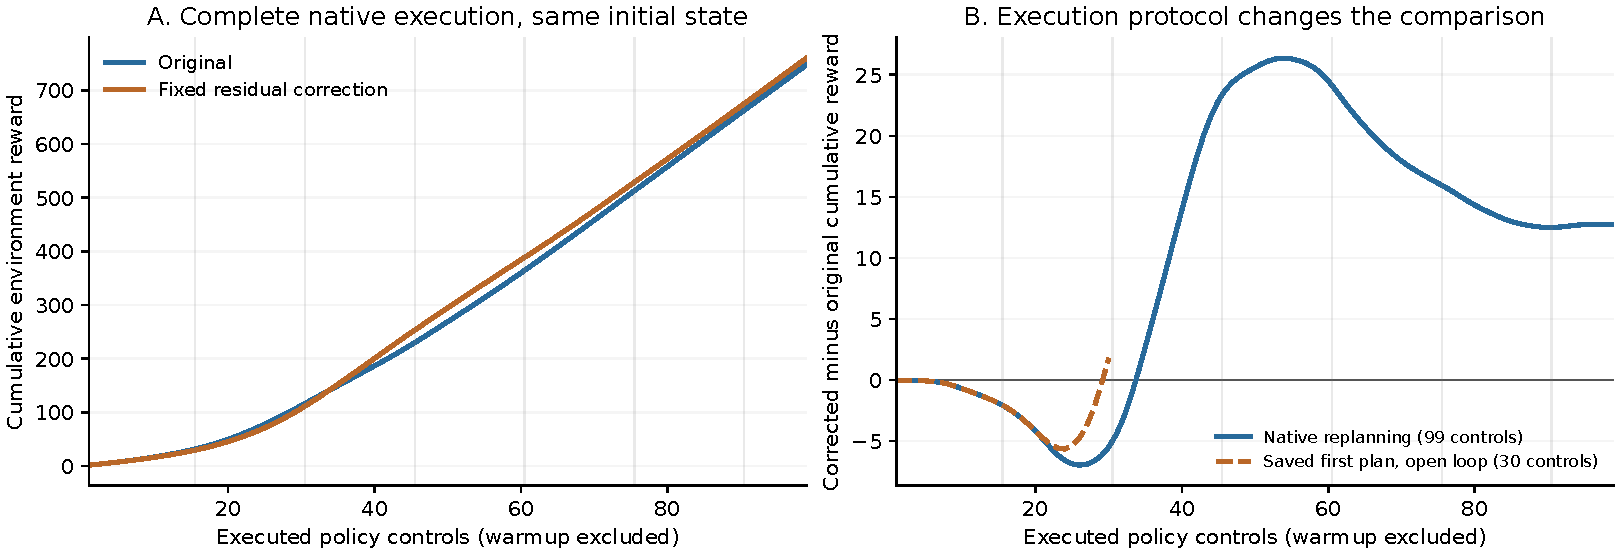
\includegraphics[width=\linewidth]{native_calibration_episode.pdf}
\caption{R004 at the same inspected root. A: complete native replanning
episodes, with 99 policy controls after one warmup control. B: fixed-bias minus
original cumulative return under native replanning (solid) and continuation of
the saved first mean for 30 open-loop controls (dashed). The shared initial
prefix does not make the subsequent continuations interchangeable. Complete
episode return improves, so the persistent-loss gate is negative. This is an
exploratory single-root comparison; initial-query forecast-error improvement
does not establish full-episode forecast accuracy.}
\label{fig:native-episode}
\end{figure}

The follow-up therefore supplies a deployable-form feature correction that
improves the declared initial-query forecast metric while reducing utility in
a fixed bank and one execution prefix, followed by a complete-episode result
in the opposite direction. It supplies neither a calibration guarantee nor
evidence of persistent return degradation. Phase 3 reuses the same inspected
root; its implementation checks are not additional independent evidence of
generality, and its complete-episode forecast accuracy has not been measured.

\subsection{A development canonicalization improves fidelity but lowers return}
Table~\ref{tab:dino} reports the fixed two-mean diagnostic. The original
prediction scores select $a_0$; canonical-request scores select $a_1$.
For both actions, canonicalization reduces weighted terminal feature forecast
MSE. Yet the independently replayed 30-control return decreases by 19.8048,
and terminal environment reward decreases by 1.9009. Neither branch succeeds
within these 30 controls, so this comparison shows no binary success loss.
The selection is made using the Goal proxy, not the forecast-error metric:
the predicted cost gap $C(a_1)-C(a_0)$ changes from $+0.265703$ to
$-0.344738$, while the actual-future proxy gap is $-0.321822$.

\begin{table}[t]
\centering
\small
\begin{tabular}{lrrrrr}
\toprule
Action & \shortstack{Original\\forecast MSE} & \shortstack{Canonical\\forecast MSE}
& \shortstack{True-future\\proxy cost} & \shortstack{Real\\return}
& \shortstack{Terminal\\reward}\\
\midrule
$a_0$: original returned mean & 1.565623 & 0.529210 & 1.701293 & 95.841823 & 5.247907\\
$a_1$: canonical returned mean & 0.958529 & 0.458303 & 1.379470 & 76.036994 & 3.347029\\
\bottomrule
\end{tabular}
\caption{One post-hoc root, two fixed actions, 30 physical controls. Forecast
MSE is measured against each action's real endpoint. True-future proxy cost
is Equation~\ref{eq:native-objective} evaluated against the original Goal;
it is not forecast error. Real return and terminal reward come from the
environment. Both actions have zero successful controls.}
\label{tab:dino}
\end{table}

\begin{figure}[t]
\centering
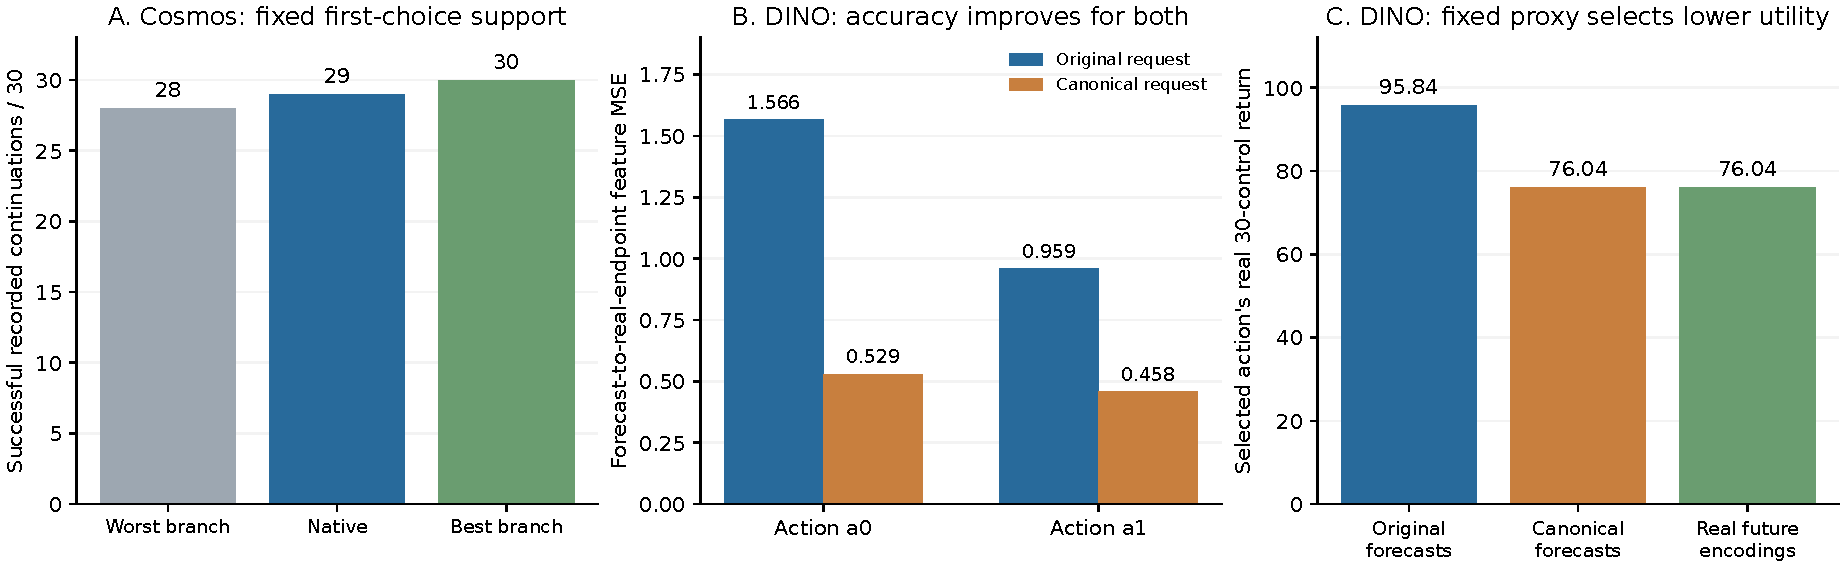
\includegraphics[width=\linewidth]{decision_diagnostics.pdf}
\caption{Two distinct decision diagnostics. A: fixed-support success limits
on Cosmos. B--C: more accurate forecasts and lower selected real return coexist
at one DINO root. The oracle-feature selector also chooses the lower-return
action. Panels B and C share the same two actions and are not independent
experiments. No population uncertainty is estimated from this single root.}
\label{fig:diagnostics}
\end{figure}

The actual endpoint features also select $a_1$. With cumulative return as
utility, the bank optimum is $U(a_0)=95.841823$ and oracle-feature utility is
$U(a_1)=76.036994$. Objective mismatch regret is 19.804829. The original
selector has zero total regret, decomposed as $19.804829+(-19.804829)$;
the canonical selector has regret 19.804829, decomposed as
$19.804829+0$. Prediction error in the original condition happens to offset
the scorer's mismatch on this bank. The negative prediction term is essential
and must not be clipped to zero or reported as a causal percentage.

This development effect is not a population estimate. The root and actions were involved
in mechanism development, and forecasts would change candidate generation
inside a full CEM rerun. Consequently, these measurements cannot identify
the behavior of a native planner equipped with an exact world model.
The companion five-action bank comes from development seed1, whereas this
two-mean bank comes from seed4. They are two distinct physical roots, but use
different candidate-construction protocols and were examined adaptively.
They cannot be pooled as a preregistered confirmation sample. On the seed1
bank, canonicalization lowers selected terminal reward from 7.699376 to
1.829723, and actual-future scoring selects the same lower-reward action.
The highest-reward action in that bank attains 7.989219. All five actions
fail the binary success criterion over the 30-control horizon.

\subsection{The proposed component-weight repair fails an offline necessity check}
The small native proprioceptive coefficient might suggest that increasing it
would fix the DINO mismatch. The measured actual-future cost differences
contradict that proposed explanation:
\begin{align}
 C_v(a_1)-C_v(a_0)&=-0.321716905,\\
 C_p(a_1)-C_p(a_0)&=-0.001053669.
\end{align}
For any $w_v,w_p\geq0$ with at least one positive,
$w_v\Delta C_v+w_p\Delta C_p<0$ in real arithmetic. Thus every nonnegative,
nonzero weighted combination still prefers the lower-return action in this
oracle-feature bank. An illustrative seven-weight grid reproduces this result;
the argument covers the entire family rather than choosing a successful
weight after inspecting test outcomes. All-zero weights give an uninformative
tie, not a calibrated scorer.

This rules out one inexpensive repair \emph{for the observed oracle-feature
ordering}. It does not rule out task-specific features, a different reward
model, nonlinear scoring, or effects on model-predicted features. It also does
not establish that scorer-side interventions outperform forecast-side ones.
Such a comparison requires separate development data, matched resource budgets,
and held-out real outcomes.

\subsection{Cosmos also contains a local prediction-side failure}
Objective mismatch is not required for every prediction-induced decision
error. At the already identified task3/init2 root, original future features
select the successful candidate, Swap features select the failed candidate,
and real-future feature substitution selects the successful one. Swap visual
latent MSE is 10.37 and 9.50 times its original value for the two candidates.
This is a local example in which larger forecast error, worse selection, and
oracle-feature recovery align.

A saved $3\times3$ factorial uses original, Swap, and real sources for visual
and proprioceptive future slots. Under each of the three proprioceptive
backgrounds, Swap visual slots select the failed branch, while original and
real visual slots select the successful branch. This identifies conditional
dependence of the frozen Value input on visual provenance at this root.
The nine cells share two historical continuations; they are not nine tasks,
new recovered episodes, or a deployable defense. Mixed feature blocks need
not describe a physically coherent future.

\subsection{TD-MPC2: separating proposal and scoring consumers}
\label{sec:tdmpc-consumer-factorial}
We test a different explanation for an existing development-case return gap:
can a dynamics update cause harm primarily by changing the policy proposals,
so that restoring the scoring path cannot recover performance?
We reuse two saved dynamics modules fitted from the random-source ($R$) and
cascade-source ($C$) \texttt{cheetah-run} trajectories at source seed 23.
$R$ is an adapted comparison model, neither the original pretrained Clean
model nor an oracle for physical outcomes. No new fitting is performed.

The native TD-MPC2 planner uses dynamics both to generate 24 policy-prior
trajectories and to evaluate its 512 candidates. We independently assign
$R$ or $C$ to these two consumers, preserving the native horizon 3,
six optimization iterations, 64 elites, stochastic action selection,
normalization, and all other original model weights.
The scoring route includes imagined-state reward readouts and terminal
policy/$Q$ evaluation; it is not a direct forecast-distance score.
Each arm executes one complete 500-control \texttt{walker-run} episode from
seed 31, with the same initial state and reset random streams.
Later states, proposal populations, and optimizer warm starts may diverge
as endogenous consequences of the intervention.

\begin{table}[ht]
\centering
\begin{tabular}{lccr}
\toprule
Arm & Proposal dynamics & Scoring dynamics & Actual episode return \\
\midrule
$RR$ & $R$ & $R$ & 612.082555 \\
$CC$ & $C$ & $C$ & 495.216321 \\
$CR$ & $C$ & $R$ & 674.885888 \\
$RC$ & $R$ & $C$ & 553.538964 \\
\bottomrule
\end{tabular}
\caption{One reused TD-MPC2 development case. Returns are sums of actual
500-control environment rewards, not planner value estimates.}
\label{tab:tdmpc-consumer-factorial}
\end{table}

Both $RR$ and $CC$ exactly reproduce the saved observations, actions,
per-control rewards, and complete returns. At the common first query,
all arms share the 24 prior first actions and all 488 Gaussian candidate
trajectories exactly; prior continuation actions can differ. Recording these
already-generated candidates preserves both CPU and CUDA random states and
adds no model evaluation.

The preregistered condition fails. Writing
$G=J_{RR}-J_{CC}=116.866234$, it requires both
$J_{RR}-J_{CR}\geq G/2$ and $J_{RC}-J_{CC}\geq G/2$.
Instead, $J_{CR}$ exceeds $J_{RR}$ by $62.803333$, while the second contrast
recovers $49.9055\%$ of $G$.
In particular, retaining $C$ proposals and restoring only $R$ scoring raises
return from $495.216321$ to $674.885888$.
The factorial interaction
$J_{CC}-J_{CR}-J_{RC}+J_{RR}=-121.125975$ also precludes an additive
allocation of the original loss to the two routes.
This counterexample does not support the proposed claim that damaged
proposal coverage prevents scoring-path recovery in this case.
It does not measure the physical quality of every candidate, demonstrate
improved forecast accuracy, or establish an attack, a defense, or a
population effect. The fixed gate is closed without a seed or threshold sweep.

SWAAP already describes poisoned world-model adaptation and the use of
TD-MPC2 dynamics for both policy-guided proposals and candidate evaluation
\cite{hu2026swaap}. Our distinction is the inference-time factorial separation
of these consumers, not a first demonstration of model poisoning or proposal
dependence. Here that separation contradicts the registered proposal-dominant
explanation. Results and the launch receipt are in
\artifact{runs/tdmpc_proposal_scoring_factorial_v1/summary.json} and
\artifact{runs/tdmpc_proposal_scoring_factorial_v1/launcher.json}; all four
physical traces and the common-first-population captures are retained.

\subsection{A complete-person ordering control in GenSafeNav}
R006 tests an explicitly added representation boundary at a learned forecast
consumer. After native prediction and feedback processing, we reverse the
visible prefix of person rows presented to the pretrained GenSafeNav actor.
Each person's current position, all forecast coordinates, and conformity
features move together; padding, visibility count, robot inputs, physical
entities, and all weights are unchanged. Inverse-permutation checks verify
that no feature values or associations are lost. This differs from assigning
one person's prediction to another person.

We reuse the existing case-0, seed-42 CPU protocol, including zero
conformity/cost noise, collision penalty $-20$, deterministic actor actions,
the CPU device bridge, and the existing native feedback indexing behavior.
Each arm retains its own normal aggregated recurrent state. The episodes
share exactly the same initial physical snapshot; later states and predictions
may diverge as consequences of different controls. No forecast-equivariance
claim is tested by the actor-only intervention.

Both complete episodes reach the goal after 119 physical controls, with no
collision and zero cumulative environment cost. Raw physical returns are
$30.185066414951063$ and $30.185057268439166$, a difference of
$-9.1465\times10^{-6}$. The registered material-loss condition---a new
collision, lost success, or at least $5\%$ return loss---is false.
The separate numerical no-effect conjunction is also false: although
terminal category, step count, and the $10^{-4}$ return tolerance agree,
the maximum paired nominal action-coordinate difference is $0.0014961064$,
exceeding the precommitted $10^{-5}$ action tolerance. We retain this failed
check and do not relabel the experiment as exact permutation invariance.

The pair completes in 17.67 seconds on CPU with 238 physical controls,
238 actor calls and 240 GST calls, including the native post-terminal
autoreset predictions. There is no training or model-API call. This fixed
intervention is closed without changing the permutation, case, seed, or
tolerances. It provides one bounded no-material-loss control, not a general
robustness theorem, proof of numerical equivalence, or validation of a common
security mechanism across systems. Full physical and presentation traces
are retained under \artifact{runs/gensafenav_person_row_permutation_v1/}.

\subsection{Duplicate removal before versus after joint forecasting}
R007 tests a restricted, researcher-added tracker-to-forecaster interface.
At each eligible GST call, we copy the lowest-index complete observed
trajectory into the lowest-index slot with no observed history, using
temporary tensors. Original valid histories, physical pedestrians, task,
weights, and direct current-state actor inputs are protected. The destination
slot need not denote the absence of a physical pedestrian. After the single
GST forward, we remove the duplicate output by restoring its invalid mask
and future XY values. The native consumer does not use its remaining
uncertainty channels, which are not claimed restored. Changes to forecasts
for other entities can still reach the actor.

Three complete case-0, seed-42 CPU episodes compare the original inputs,
this single duplicate with output removal, and exact removal before GST.
The last arm restores the original input tensor before forecasting; it is
a controlled reversal of this exact operation, not a general defense.
The inherited native evaluation settings are the same as in R006.

\begin{table}[ht]
\centering
\begin{tabular}{lrrcc}
\toprule
Condition & Physical return & Controls & Success & Collision \\
\midrule
Original & 30.185066415 & 119 & Yes & No \\
Duplicate, remove output & 30.087496792 & 102 & Yes & No \\
Remove before GST & 30.185066415 & 119 & Yes & No \\
\bottomrule
\end{tabular}
\caption{R007 complete physical episodes. All three have zero cumulative
environment cost. The duplicate arm reaches the goal sooner; its small
return decrease is not a material-harm result.}
\end{table}

The duplicate arm contains 98 eligible, actually consumed interventions.
At the first common eligible call, original history inputs and direct actor
current-state fields agree, while forecast XY for original valid entities
changes by up to $0.0095983$. This is a local influence diagnostic, not a
forecast-to-truth error or an attack-success metric. Full-episode return
changes by $-0.0975696$ ($-0.3232\%$), below the precommitted loss threshold
of $1.5092533$; neither collision nor loss of success occurs. Thus the
registered material-harm gate fails. Pre-GST removal reproduces the entire
original physical trace, actor observations, resets, forecasts, and outcome
exactly, but recovery alone cannot turn the failed harm gate into a positive.

The test completes in 27.11 seconds, with 340 physical controls and 343 GST
calls including three post-terminal reset predictions, without API calls or
training. We close this fixed operation without changing the source rule,
duplicate count, task, or seed. This single reused case establishes neither
external attacker access nor a shared three-system security mechanism.
The execution snapshot, per-call tensors and complete physical records are
in \artifact{runs/gensafenav_forecast_track_duplicate_v1/}.


\section{Discussion and remaining tests}
\label{sec:discussion}
\paragraph{What the evidence changes.}
The Cosmos table makes a large first-choice success-harm claim impossible on
the already measured support, while preserving the one observed local loss
and cost sensitivity. The DINO development bank rejects a worsened-terminal-MSE
explanation for its return loss and identifies a scorer mismatch that scalar
component reweighting cannot repair on those two actions. The 30-root
confirmation establishes lower mean utility after offline oracle substitution
for a fixed bank transferred from development. Its original ranker also trails
two fixed-action baselines, making limited selector competence part of the
result. The R003 native mean-versus-elites check is negative. The R004 fixed
correction supplies an exploratory, deployable-form prediction change, but
its single native query has opposite utility directions at H15 and open-loop
H30. The subsequent complete native episode has higher corrected cumulative
return, so its persistent-loss gate is also negative.
These are interface-specific diagnoses. None implies
that all attacks fail, that prediction accuracy is irrelevant, or that all
world-model agents are objective-limited.

\paragraph{What the confirmation does and does not test.}
The completed protocol fixes roots, candidate construction, utility, scorer,
tie handling, and the oracle comparison before confirmation. It tests the
paired utility contrast directly; positive oracle mismatch alone would not
have sufficed. The negative interval supports the specified average effect
for this bank and root-generating procedure, despite 18 utility ties. The
oracle's feature accuracy is guaranteed, while its availability is diagnostic
only. The later fixed-bias test avoids evaluation truth as a correction input,
but reuses already examined roots and cannot inherit the oracle test's
confirmation status. A new confirmation of this correction would require
disjoint, prespecified roots and both actual forecast-error and utility
measurements. Independent confirmation across task families and native planning
interfaces remains unexecuted.

\paragraph{Native planning versus an added ranker.}
A low-cost fixed-bank diagnostic is useful for isolating the scoring question.
Both the DINO two-mean comparison and the 30-root panel use added rankers;
a fixed bank that is the actual native selector's support can retain its native
interface designation. A native CEM test must record the actual
proposal updates and returned mean, evaluate any newly returned executable
sequence in the environment, and specify whether its claim concerns a frozen
population or a changed full planning process. Holding only the final elites
fixed does not reproduce native CEM or include the returned mean automatically.
R003 and R004 phase 2 now record and replay native means explicitly. R004's
later proposal populations differ between conditions, so its prefix result
cannot be attributed solely to a different final ranking on fixed actions.
Moreover, H30 open-loop continuation improves while H15 worsens. The separately
measured complete episode with native replanning also improves in primary
return, despite later first success. These results show why a prefix or
open-loop continuation cannot stand in for a complete native episode.

\paragraph{Defenses and generalization.}
Oracle futures are an offline instrument, not a deployment defense. An eventual
scorer-side repair must be fitted on development data and compared with a
prespecified forecast-side correction on disjoint roots. Report absolute
utilities for each condition, including normal-input behavior, rather than
only the gap between conditions. An independent task family is needed before
the observed phenomenon can be described as general across tasks or models.
The fixed-bank oracle protocol has been executed in full, and two single-root
native-query follow-ups and a complete-episode pair are reported separately.
A trained-scorer comparison and independent confirmation of the fixed correction
are not established by these single-root or reused-root results. Proposed
forecast-service integration permissions are assumptions to test, not evidence
of an existing native attack surface.

\section{Limitations}
The empirical evidence remains uneven across systems and interfaces.
Cosmos's finite support is complete for a first-choice diagnostic, not for
its full closed-loop action space. The DINO confirmation has 30 independently
reset roots from one task family and a bank of five development-derived
sequences, shared across those roots. This isolates the added scorer's choices
but does not sample fresh native CEM proposals or establish full closed-loop
performance. Candidate count, mixture grid size, repeated rendering, and
factorial cells cannot enlarge the independent sample size. The earlier
post-hoc development banks do not enlarge the confirmation sample either.
Project-held-out seeds do not establish a holdout from model pretraining.
The original ranker's lower mean utility than two fixed candidates limits
claims about normally competent planning; a scorer trained and validated on
separate roots has not been tested.

R004 phase 1 is an exploratory reuse of the 30-root panel. Its correction
improves candidate-averaged error, not every candidate's error, and carries
no statistical calibration guarantee. Phase 2 contains one fresh root and
one planning query per condition. Its error diagnostic covers only the two
returned means, while later CEM proposals differ. The H15 reward and return
loss reverses at open-loop H30. Phase 3 completes both native episodes at the
same already inspected root and finds higher corrected 99-control return;
the preset persistent-loss condition is absent. Later first success and better
final success point in different directions and remain secondary to that
endpoint. Initial-query MSE improvement does not establish full-episode
forecast accuracy, and the full episode is not an independent-root replication.
The expanded H15 return criterion was added after
launch and before replay outcomes; this timing must not be represented as
prelaunch registration. R003's negative result is retained without replacing
its root. None of these follow-ups establishes a distinct external security
mechanism or a third independent affected system.

The actual-future representation is limited to the model's observation and
encoder; oracle-feature scoring need not expose a physical state or an optimal
reward representation. Zero oracle error is a constructed manipulation check,
and intermediate mixtures may be off the feature manifold. Endpoint accuracy
need not measure path accuracy, and terminal proxies need not optimize cumulative
return. The prospective primary endpoint is terminal reward and decreases along
with cumulative return, so that result is not only a cumulative-versus-terminal
metric distinction. Success is sparse (2/30 versus 0/30) and descriptive; the
dense-reward result is not a broad claim of induced task failure.

The interface bounds depend on complete recorded support, matched continuation
policies, and the stated outcome definition. A change that produces a new mean
action, changes later controls, or changes an environment's hidden-state
distribution is outside them. One realized stochastic branch per candidate
does not provide a bound on its expected return. Full mediator identification,
attacker reachability, and deployment permissions require additional evidence.
The archival source includes systems with incompatible, retired, or incomplete
protocols; these cannot be pooled into a seven-system replication claim.

\section{Conclusion}
Fixed-support utility tables and actual-future scoring answer two questions
that forecast error alone cannot: how much the measured decision interface can
change real outcomes, and whether its frozen objective would choose well given
the observed futures. The Cosmos cache bounds first-choice success loss on its
measured support. A completed 30-root DINO confirmation shows that offline
actual-future substitution lowers mean terminal reward by 1.542393 in an added
five-action ranker, while simple fixed choices outperform its original scoring.
A fixed additive correction reproduces a smaller exploratory effect without
evaluation futures as correction inputs. Its native single-query comparison
reduces H15 reward and return but improves both under H30 open-loop continuation.
Complete native replanning at that same root increases 99-control return by
12.738701, while delaying first success; the preset persistent-return-loss
gate is negative, as is the native elite-mean gate. Together these findings
support a reproducible diagnostic study of a known prediction--control mismatch,
with an explicit negative full-episode result for the proposed loss extension.
They establish neither a new security mechanism nor independent cross-task
generality, full-episode forecast-fidelity improvement, or a validated repair.

\bibliographystyle{plain}
\bibliography{references}

\appendix
\section{Evidence ledger and reproduction}
\label{sec:artifacts}
Paths below are relative to the repository root. The paper build uses cached
numerical analyses and does not call a model API. The repository's earlier
knowledge-base update and this manuscript may be newer than the public GitHub
baseline; the artifact manifest records content hashes rather than assuming
that a branch name identifies the current working tree.

\begin{description}[style=nextline,leftmargin=0pt]
\item[Finite-support aggregation]
\artifact{scripts/compute_decision_leverage_panel.py}, with generated
\artifact{reports/decision_leverage_paper/panel_*} outputs. Includes explicit
eligibility and exclusion reasons; incomplete systems are not assigned zero
leverage.
\item[Cosmos actual branch outcomes and bounds]
\artifact{runs/cosmos_first_candidate_utility_recovery_analysis_v1/analysis.json}\\
\artifact{reports/cosmos_first_choice_identifiability_bounds_20261015.json}\\
\artifact{reports/cosmos_first_selection_mediation_20261015.json}.
\item[DINO measured H30 countercheck]
\artifact{reports/dino_first_query_terminal_truth_decision_20261015.json}\\
\artifact{scripts/analyze_dino_first_query_objective_decomposition.py}.
\item[New objective-family calculation]
\artifact{scripts/analyze_decision_objective_reweighting.py}\\
\artifact{reports/decision_leverage_paper/objective_reweighting.json}.
\item[Cosmos actual-future and modality controls]
\artifact{reports/cosmos_first_query_truth_decision_20261015.json}\\
\artifact{reports/cosmos_future_modality_factorial_decision_20261016.json}.
\item[Completed prospective DINO confirmation]
\artifact{configs/decision_leverage_dino_e1.json}\\
\artifact{reports/decision_leverage_paper/prospective_dino.json}\\
\artifact{runs/decision_leverage_dino_cpu_confirmatory/}.
The design configuration records the planned protocol and retains a prelaunch
execution-status field. The completed analysis JSON is the execution evidence:
all 30 registered roots are included, calibration roots are excluded, and its
validation record reports source bindings and verified raw artifact hashes.
It contains the paired bootstrap summaries, all mixture arms, baselines,
activity receipt, and interpretation limits. Optional scorer-training roots
remain unexecuted. The later native-query follow-ups below have their own
protocols and do not enlarge this confirmation sample.
\item[Negative native elite-mean gate, R003]
\artifact{runs/cem_elite_mean_utility_gate_v1/summary.json}.
Records the unchanged native query, all eleven real prefix outcomes, exact
mean/elite consistency checks, and the absent primary condition.
\item[Fixed residual correction, R004 phase 1]
\artifact{runs/forecast_residual_calibration_v1/fit_commitment.json}\\
\artifact{runs/forecast_residual_calibration_v1/summary.json}\\
\artifact{reports/forecast_residual_calibration.json}.
The saved bias predates evaluation reads. The full report retains all 30
reused roots and the stronger fixed-action baselines; inference is descriptive.
\item[Native residual-correction query, R004 phase 2]
\artifact{runs/native_forecast_calibration_gate_v1/summary.json}\\
\artifact{runs/native_forecast_calibration_gate_v1/interpretation.json}.
The interpretation records the after-launch, before-outcome criterion addition
and the opposite H15/H30 utility directions. These files are not evidence of
a complete episode; the subsequent episode experiment is recorded separately.
\item[Complete native episodes, R004 phase 3]
\artifact{runs/native_forecast_calibration_episode_v1/summary.json}\\
\artifact{runs/native_forecast_calibration_episode_v1/raw/result.json}\\
\artifact{runs/native_forecast_calibration_episode_v1/calibrated/result.json}.
Each arm also retains its 99-step \artifact{trace.jsonl}. The first query
exactly repeats phase 2 as an implementation check. The complete-episode
cumulative-return loss condition is false; no full-episode forecast-error
claim is recorded. The figure is
\artifact{reports/decision_leverage_paper/native_calibration_episode.pdf},
with its companion source ledger.
\end{description}

\section{Utility and interface reporting requirements}
\begin{table}[h]
\centering
\small
\resizebox{\linewidth}{!}{% Generated by scripts/compute_decision_leverage_panel.py; sums over fixed roots.
\begin{tabular}{llrrrr}
\hline
System / interface & Utility & Roots & Range & Baseline & Harm cap \\
\hline
Cosmos & Success count & 30 & [28, 30] & 29 & 1 \\
Cosmos & Capped steps & 30 & [3230, 3646] & 3477 & 169 \\
DINO-WM & 30-step return & 1 & [24.23, 110.152] & 109.057 & 84.827 \\
DINO-WM & Terminal reward & 1 & [0.481, 7.989] & 7.699 & 7.218 \\
DINO-WM & 30-step success & 1 & [0, 0] & 0 & 0 \\
WorldAgen & 3-step success & 3 & [0, 0] & 0 & 0 \\
WorldAgen & 3-step reward & 3 & [0, 0] & 0 & 0 \\
\hline
\end{tabular}
% DINO is an added fixed-bank selector, one root. WorldAgen is only a local utility diagnostic:
% three roots share one episode and no forecast-driven selector was run.
% Harm cap is baseline-specific; lower is better only for capped steps.
}
\caption{Generated archival finite-support panel. DINO uses the seed1 five-action
development bank and an added ranker. WorldAgen supplies three short roots
from one episode and no forecast-driven native selector; its zero three-step
task reward is a local metric observation, not evidence of full-task robustness.
Systems lacking eligible real continuation tables are excluded rather than
assigned zero bounds. The separate completed 30-root DINO confirmation is
reported in Table~\ref{tab:dino-prospective}.}
\end{table}
Every new record should identify the originating episode, task, root state,
environment and wrapper versions, original task Goal, model checkpoint,
candidate bytes or content hash, noise and continuation settings, native or
added selector status, forecast horizon, execution horizon, and tie rule.
Report success, dense return, terminal reward or distance, and capped cost
only where their definitions are available. A missing utility is missing,
not zero. Preserve the predeclared primary measure when secondary metrics
disagree, and show all retained measures so that harm cannot be manufactured
by choosing a favorable metric after inspecting the result.

\end{document}
